Figure \ref{fig:gfp-pcc-predictions} presents the result of training with PCC loss on intensity images. The model convergence and visual comparison between ground truth and predictions is displayed. One can see that some of the cells are present in predictions, but are missing in ground truth images. These are dead cells that do not express GFP anymore, however the cell body is still present in DIC. An additional observation is that the boundary is generally more blurry than in ground truth fluorescence, which is typical for all previous organelles as well. However, all cells are clearly visible and can be separated using additional image postprocessing pipelines.
\begin{figure}[H]
	\begin{center}
		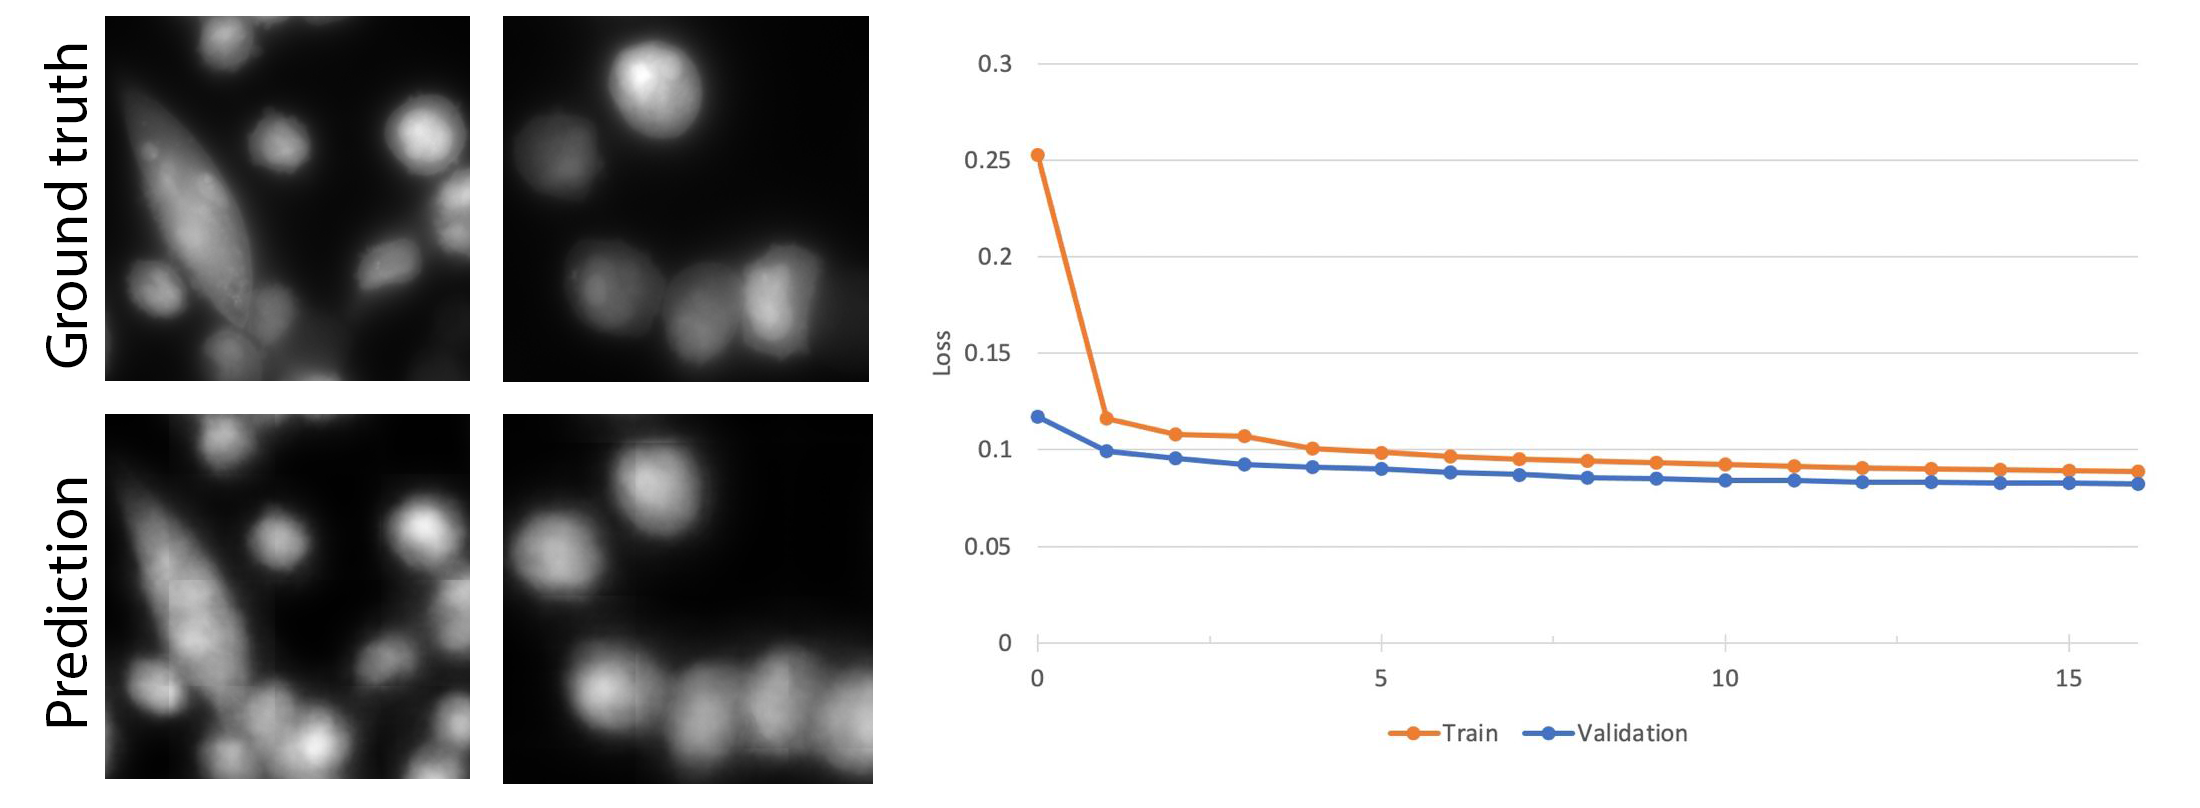
\includegraphics[width=0.6\linewidth]{bilder/gfp/predictions.png}
		\caption{Training with Pearson correlation loss}\label{fig:gfp-pcc-predictions}
	\end{center}
\end{figure}

In Figure \ref{fig:gfp-bce-predictions} we can see the results of training on the binarized image dataset. The model converges and the predictions are successful as well. Without the intensities it might be more difficult to visually separate the cells from the mask, as opposed to the image with intensity values. The predicted masks are not binarized yet contain continuous values from the interval $[0, 1]$. The following observation shows how the model generalizes: preprocessed ground truth image still has not very strict boundaries in its masking even after local thresholding binarization. After zooming in one can see that some that the boundaries of some cells were oversegmented. This happens due to the different intensity values for different cells. However, this is not a an issue as the model is still able to generalize well and predicts the middle part of the cell confidently, then smoothly reduces the confidence on the cell boundary. After thresholding such predictions one can choose such a threshold that will get just enough of the cell boundary needed. In our case the value was chosen to be $0.8$.

An interesting detail here are dead cells mentioned above. They are present in DIC, but do not express GFP. One can see a clear example of such cells selected with green circles in Figure \ref{fig:gfp-bce-predictions}. The model generalizes in a way that it continues to segment all of the cells regardless of their state. This is an expected behavior as the amount of dead cells in the dataset is pretty low and occasional mistakes do not push the model strong enough to be able to learn the features that separate dead from living cells. We proceed with the existing model for futher evaluation, however it might be useful for further research to address this issue. For example, \cite{Christiansen_2018} has demonstrated the ability of their model to differentiate dead cells from alive ones by staining the dead ones and then training the model to differentiate between them. 

\begin{figure}[H]
	\begin{center}
		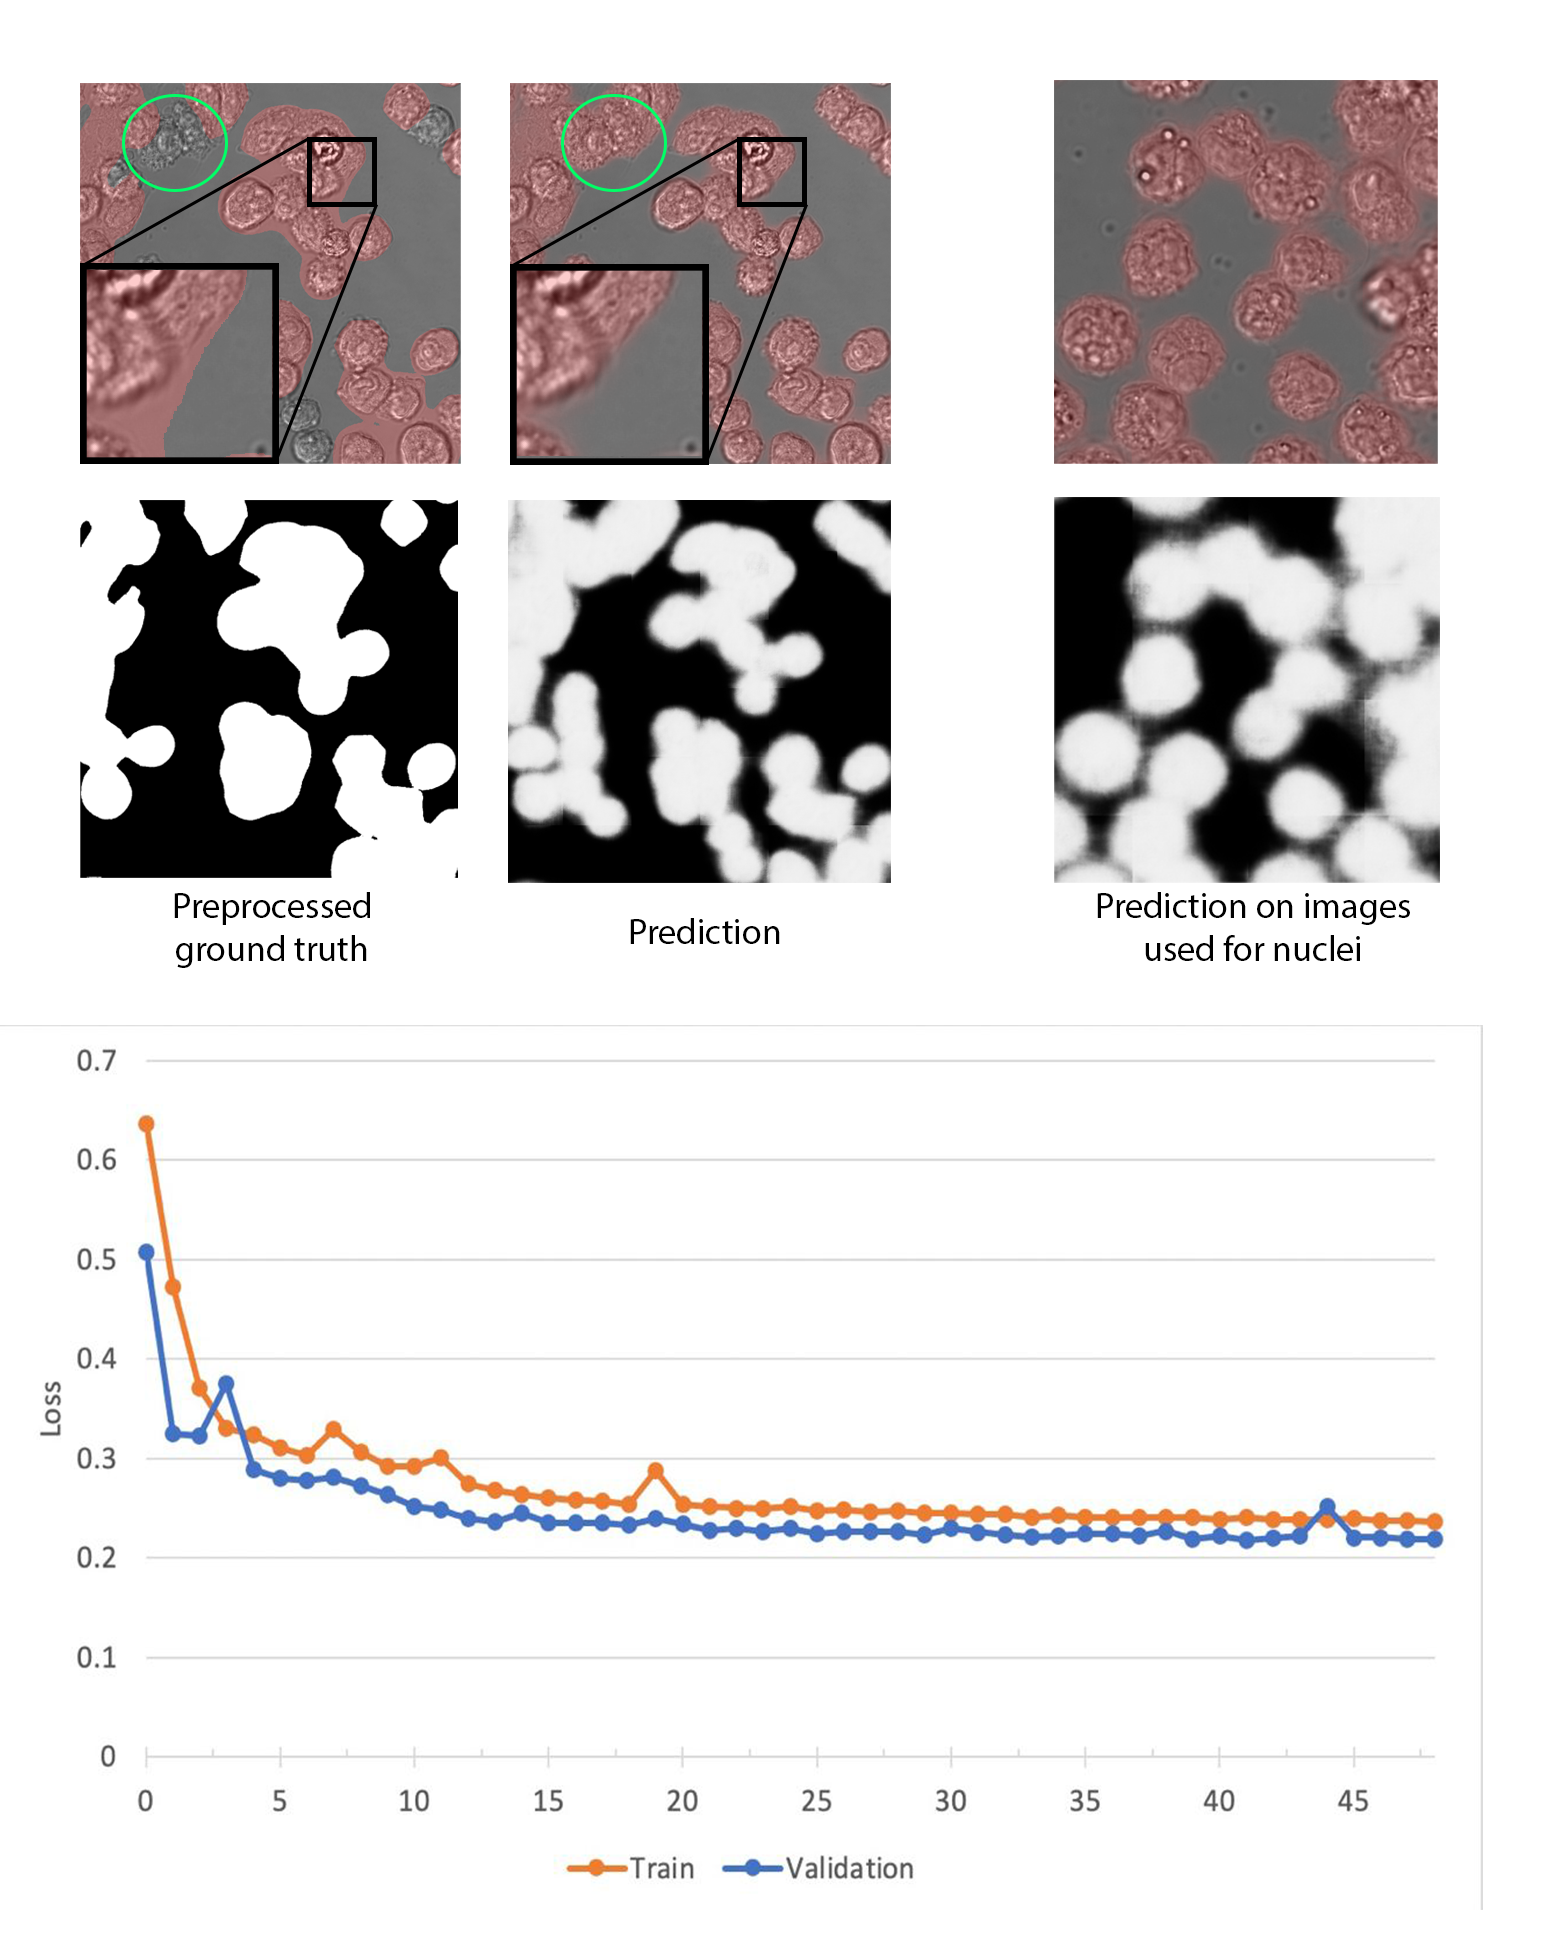
\includegraphics[width=0.8\linewidth]{bilder/gfp/binary-bce/enlarged.png}
		\caption{Training with BCE loss}\label{fig:gfp-bce-predictions}
	\end{center}
\end{figure}
